\chapter{Tasks Undertaken}
Throughout the course of the internship, a variety of tasks were undertaken and completed.  
For the sake of brevity a small subset of the most interesting of these tasks are outlined below. 

\section{Rebuilt DNS Management System}
DNS plays an important part in sending emails. As discussed in \refsec{sec:DNS}, there a several DNS records that must be maintained for a server to send email. As HubSpot aims to offer as seemless an experience as possible to its customers, it attempts to take care of as much of the DNS settings as possible on behalf of the customer. Ultimately however, if a customer want's HubSpot to send their marketing emails through an SMTP domain of \java{emails.company.com}, these DNS records must be obtainable at that domain as discussed in \refsec{sec:DNS}. 

As things change at HubSpot, it is quite likely that these DNS records would need to change over time. For example, if the customer should add another dedicated IP address to their account, this would have to be added to their SPF record. At first glance this would require HubSpot's customers to be frequently changing their DNS records, something most customer's would not be overly comfortable with. The solution to this problem, as with so many problems in computer science, is indirection. 

The Domain Name System supports the concept of including other DNS records, even from entirely different domains. This is exactly the behavior that lets HubSpot manage their customers' DNS on their behalf. For example, instead of \java{emails.company.com} having the SPF record which contains their allowed sending IPs and having to change it should their sending IPs change, they can simply setup this record as a pointer to another DNS record, a record on HubSpot's domain. Clients who require the SPF record for for \java{emails.company.com} will be informed to use the record contained on HubSpot's domain instead. An example of this is shown in \reffig{fig:dnsIncludes}, where 99 is the customer's HubSpot identification number. A similar setup exists for customers' DKIM records.

Thus, the customer only ever needs to set up the DNS pointers to HubSpot's domain once. Once that is done, HubSpot can control the actual values of those DNS records on behalf of the customer. 

\begin{figure}[H]
      \centering
      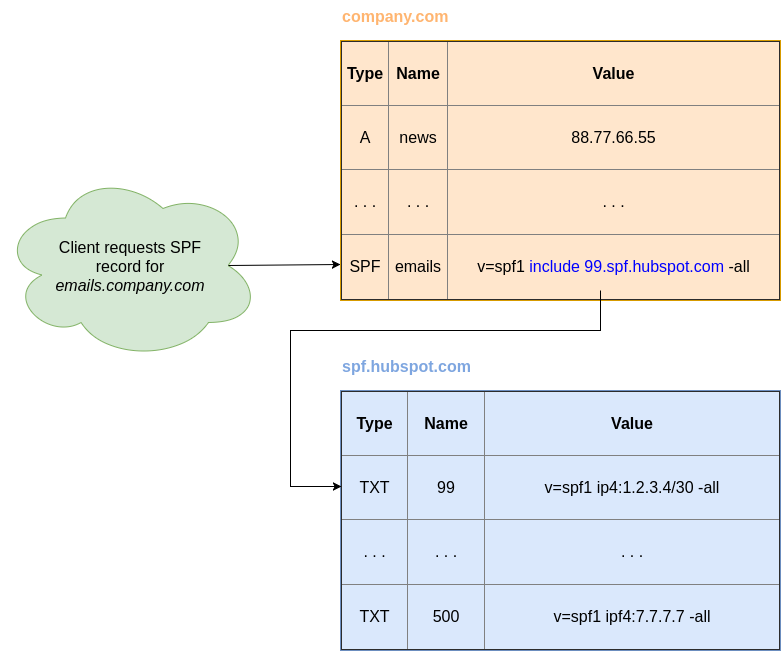
\includegraphics[width=0.8\textwidth]{renders/DnsIncludes.png}
      \caption{DNS Includes for \textit{emails.company.com}, HubSpot Customer 99.}
      \label{fig:dnsIncludes}
\end{figure}

Initially, all the DNS records that the customers include were created at various points in the code. There was no definition for exactly what DNS records should be available and where they should be available for a given account. Some of the DNS record creation was coupled to the code that was responsible for creating new customer accounts, but as time went on, different DNS records were required, resulting in redundant DNS records being created. There were also several cron jobs (jobs which run on a schedule) responsible for checking the current status of the DNS records and attempting to adjust them as necessary. There was also no unit tests for any of the code which synced DNS records. Some of these jobs concluded that different values should exist for the same DNS record, resulting in the jobs competing with each other and updating DNS records every time they ran. It was also unclear what DNS changes were required if accounts were updated. This led to the creation of an entirely new DNS management system.


\subsection{Requirements for the Management System}
Prior to beginning to rebuild the system, an analysis of the current system was required to ensure all the required functionality contained in the old system would be included in the new system. Another important step was to consider what the \textit{ideal} system would look like. There were two main options to consider:

\begin{enumerate}
    \item{Create all the DNS records required when the corresponding customer account was created. As discussed previously, it is likely that the value of these DNS records would change over time. Thus, this would also require periodic cron jobs in order to compare the current state of a customer's DNS records against what the system believes their DNS records should be and to update them accordingly. The downside to this approach was having the required DNS records defined and maintained in two separate places - once during account creation and once during the DNS record synchronization.}
    \item{Abstract away all DNS record creation from the account creation process and write the periodic cron jobs in such a way that they can also create brand new DNS records as necessary. The downside of this approach is that there would be a period of time in which the accounts would be created, but have invalid DNS records, which could be problematic if not managed appropriately.}  
\end{enumerate}

After some consideration, it became clear that option two was the better choice. The period of time in which the accounts would be created but have invalid DNS records could be managed rather simply. Provided the jobs were written correctly, this approach would have the benefit that it could sync DNS records for arbitrarily complex entities. For example, initially the customer's account was all that was required in order to keep their DNS records in sync. However as time went on, other types of DNS records also needed to be maintained, which could not necessarily be deterministically generated from just a customer's account. An example of this is IP addresses which are owned by HubSpot, but not yet in use by any customer. These IP addresses should have specific DNS records in place. However by definition, these IP addresses are not yet assigned to any accounts. Thus, the new system should also be able to sync DNS records based on IP addresses. In the past the solution to this problem would have been to simply create yet another periodic cron job to maintain those DNS records, making it even more difficult for an engineer to know where in the code a given DNS record is maintained.

Another important concept are DNS \textit{zones} (sub domains). For easier organization and management of a large number of DNS records, a top-level-domain (TLD) can be further sub-categorized into zones. In the previous example domain \java{emails.company.com}, the TLD is \java{company.com} and a zone on that TLD could be created for \java{emails}. The purpose of DNS zones is to allow finer grained control for a domain with a large number of DNS records. For example, a customer could setup all the records required for HubSpot's email marketing on a single zone, the \java{emails} zone, isolated from all the domain's other records (e.g. for their website, internal email etc). 

The requirements of the new system were determined to be the following:
\begin{enumerate}
      \item{It can sync DNS records for arbitrary entities (Accounts, IP Addresses etc)}
      \item{The code for generating the values of specific DNS records should be decoupled from the code which actually runs the job. This allows for comprehensive unit testing of the code which generates the records.}
      \item{It should only make external requests to update records which are no longer valid.}
      \item{It should group the records required for a given entity by zone, allowing for easier record lookups and updates}
\end{enumerate}

\subsection{Implementation of the System}
The first task was to decide how the code which builds the DNS records should be organized. It was imperative to have this code be as clear and concise as possible. The DNS records themselves are hosted on various providers (e.g. Cloudfare), but the Platform team in HubSpot provides a simple client for working with these records (creating records etc). A \java{DnsRecordBuilder<T>} interface was defined and is shown in \refapp{appendix:dnsManagement} \refcode{lst:dnsRecordBuilder}. This interface defines the following methods:

\begin{itemize}

      \item{\java{Multimap<String, RecordRequest> buildSpfRecords(T entity)}}
      \begin{itemize}
            \item{This method will generate the SPF records required for a given entity of type \java{T} (e.g. an account)}
            \item{Equivalent methods are also defined for MX, A and DKIM records}
            \item{The \java{RecordRequest} object is a Java object whose contents can be passed to the DnsClient library to create / update / delete the given record}
            \item{These methods return Multimaps (which is essentially a \java{Map<String, Collection<RecordRequest>>}) which use the record's zone as the key}
            \item{All these methods are defaulted to returning empty multimaps (if they are not overridden)}
      \end{itemize}

      \item{\java{boolean appliesTo(T entity)}}
      \begin{itemize}
            \item{This method specifies whether or not this particular implementation of \java{DnsRecordBuilder} should apply to this entity}
            \item{For example if the entity was an account, this method can be used to specify that only accounts with dedicated IP addresses should use this \java{DnsRecordBuilder}}
      \end{itemize}

      \item{\java{Map<String,DnsConfiguration> getDnsConfigByZone(T entity)}}
      \begin{itemize}
            \item{The \java{DnsConfiguration} is a Java object which contains a zone name and a list of \java{RecordRequest} objects (which contains all the records to be created)}
            \item{This method has a useful default implementation which aggregates all the multimaps returned by each methods that builds the records of each type (SPF, DKIM, A, MX) into a single multimap. The returned map of DNS configurations by zone can then be built and returned.}
            \item{This is the most common method called on this interface as it invokes all the other methods, returning the exact DNS configurations (by zone) needed to keep the given entity up to date.}
      \end{itemize}

      \item{\java{Map<String, String> buildPtrRecords(T entity)}}
      \begin{itemize}
            \item{The final method defines the PTR records that should be created for this entity, returning a map containing the IP address as the key and the host name corresponding to this IP address as the value}
            \item{As discussed in \refsec{sec:DNS}, PTR records are used to perform reverse A lookups, defining the host name associated with an IP address.}
      \end{itemize}
\end{itemize}

Implementations of this interface can then be created for a given entity type. For example, a \java{DefaultAccountDnsRecordBuilder<Account>} was created to encapsulate all the records that need to be created for every HubSpot customer account. Similarly, a \java{UnassignedIpDnsRecordBuilder<IpAddress>} was also created to encapsulate all the DNS records required for an unassigned IP address. The \java{IpAddress} object contains the status of the IP address (whether its associated with a customer account or not). The \java{appliesTo} method of this implementation can then check this field and only return DNS records if the \java{IpAddress} is in fact unassigned. As time went on, more of these \java{DnsRecordBuilder} implementations were created, encapsulating different DNS requirements. This provides a very clean and extensible way of defining DNS records which are deterministically built from arbitrary entities.

The next step in the implementation was to write an intermediate class which given an entity of type \java{T}, applies all the \java{DnsRecordBuilder}s corresponding to the entity and finds out which records need updating. 

A \java{Map<Class, List<DnsRecordBuilder>>} is created and is used to determine the list of \java{DnsRecordBuilder}s that need to be applied to a given entity by simply looking up the entity's class in the map. The \java{getDnsConfigurationsByZone} method defined above is invoked on each of the builders in the list, generating all the DNS records that need to be present for the given entity. 

Finally, another piece of logic was written to determine which records need to be updated for the entity. This is done by checking the records against an in-memory cache, a database cache and finally live DNS. This reduces the number of real DNS queries that need to be made. The in-memory cache and database cache would be frequently invalidated to ensure cached DNS records had not become stale. Any records which require updates are then added to a \java{List<DnsConfiguration>} and returned to the caller to perform the actual updating. This code segment is provided in \refapp{appendix:dnsManagement} \refcode{lst:recordBuilderApplier}.

The final step was to create the cron job which will use the above code to keep the required DNS records in sync. The HubSpot development platform provides a simple means of registering jobs which are to be run on a schedule. The benefits of the extra complexity of the above code are seen in the implementation of the job. The job simply fetches all the entities of interest (\java{Account}s, \java{IpAddress}es etc) from a database. For each of these entities, the job calls the method from the intermediate class as discussed in the previous paragraph using the entity as a parameter. This method returns the list of records which need be updated or created. The job then handles performing the required DNS updates. A simplified version of the job in which the DNS records for all accounts are synced is shown in \refapp{appendix:dnsManagement} \refcode{lst:dnsSyncJob}.

\break
\section{CIDR Minimization Algorithm}
As discussed in \refsec{sec:DNS}, SPF records are a vital part of authorization when it comes to sending emails. SPF records are typically used to specify a set of IP addresses that a particular domain may send emails from. An important aspect of SPF records (or more specifically, the underlying TXT record) is that the length of the entire record value (which is a simple string) should be at most 255 characters as per RFC 7208 \cite{spfRFC}. Given the fact that a particular HubSpot customer may potentially send email over any one of tens of HubSpot owned IPs, this can cause problems. 

One of the upgrades customers can avail of is purchasing dedicated IP addresses, which will be used for their email traffic and theirs only. This allows the customer to build up a good IP reputation without the risk of the reputation being harmed by other HubSpot customers who may send lower quality email. HubSpot owns a large number of IP addresses in order to facilitate this. One of the other tasks undertaken during the internship was automating the process of setting up email sending accounts for new dedicated customers. Prior to this automation, one of the decisions that needed to be made by support staff working with customers was which IP address(es) to assign to customers. Some customers have existing IP addresses and IPs should be selected in order to minimize the length of the resulting SPF record that the customer will have. SPF records support CIDR notation (see \refsec{sec:CIDR}) of IP addresses, meaning smart IP selection can save valuable characters in a customer's SPF record. Thus, an important step in automating the setting up of customer accounts with dedicated IP addresses was automating the IP address selection, while still minimizing the resulting SPF records.

\subsection{CIDR Notation} \label{sec:CIDR}
CIDR (Classless Inter-Domain Routing) notation is a compact way to represent an IP address along with its associated subnet mask and network prefix \cite{cidr}. With regards to SPF records, it is useful as it can be used to compactly represent a set of IP addresses. This set consists of the IP addresses of all the hosts on the sub-network (subnet) specified by the network prefix. This section will primarily discuss CIDR notation for version four (IPv4) IP addresses, though all the same logic holds for version six (IPv6) IP addresses. 

Typically, IP addresses are represented as quartet of period separated integers ranging from 0 to 255, for example, $192.168.1.1$. However, this representation is simply employed in order to make reading IP addresses easier for humans. In actuality, version four IP addresses are more simply represented as 32 bit integers. Each of the numbers in the quartet can take on one of 256 values. Thus:

\begin{equation}
\begin{split}
\log_2 256 = 8\,bits\,per\,element\,in\,quartet \\
8\,bits\,per\,element \times 4\,elements\,in\,quartet = 32\, bits
\end{split}
\end{equation}



$192.168.1.1$ could be represented as a 32 bit integer by using $192$ as the upper (most significant) 8 bits, $168$ as the next 8 bits and so on. CIDR notation contains the IP address in question, followed by a slash and a number, for example $192.168.1.2/31$. CIDR notation partitions the 32 bit representation of the IP address into two pieces - the upper bits make up the network prefix and the remaining bits are used to specify the specific host on that network. The number following the slash denotes the number of bits to use for the network prefix. Thus, $192.168.1.3/31$ specifies that 31 out of the 32 bits should be used for the network prefix and all other bits should be zeroed in order to obtain the network address. This implies that the network address is $192.168.1.2$. This is because the least significant byte of this IP address is 3, or $(0000\enspace0011)_2$ in binary, and the last bit is to be zeroed meaning the last byte of the network address becomes $(0000\enspace0010)_2$, which is 2 in base-10. 

CIDR notation can thus be used to represent a set of IP addresses, provided they are contiguous. The set has a cardinality that is an integral power of 2 and the first IP address in the set lies on a CIDR boundary. The set of IPs $\{192.168.1.0,\enspace192.168.1.1\}$ can be represented using CIDR notation as $192.168.1.0/31$. The logic here is that the address of the subnet containing the hosts of interest is provided and the implied set of IPs is the set of all IP addresses of the hosts on that subnet.  Thus, if a customer owns these two IP addresses, their SPF record can simply contain the CIDR notation value of the subnet which contains the two IP addresses, reducing the number of characters required by almost half. This is due to the fact that $/31$ implies that there is one bit (the last bit) which identifies the host on the subnetwork defined by $192.168.1.0$. This bit can either be a zero or a one, yielding the two possible IP addresses that were started with - $192.168.1.0$ or $192.168.1.1$.

\subsection{A Simplified Version of the Algorithm}
The main objective of the algorithm is summarized as follows (Note if the CIDR post fix is omitted, $/32$ is implied): \hfill\break\break
Given a set of existing IP addresses $S_e$ (the \textit{existing} set) and a set of available IP addresses $S_a$ (the \textit{available} set), choose a set of $n$ IP addresses $S_c$ (the \textit{chosen} set) from $S_a$ such that the resulting number of characters in the CIDR representation of $S_f$ (the \textit{final} set) is minimized, where 

\begin{equation}
S_f = S_e \cup S_c
\end{equation}

An example scenario in which the algorithm could be used is given in \refeq{eq:ipAlgExample}
\begin{equation}\label{eq:ipAlgExample}
\begin{split}
 &   S_e = \{1.1.1.1,\enspace1.1.1.2\} \\
 &   S_a = \{1.1.1.0,\enspace1.1.1.3,\enspace1.1.1.4,\enspace1.1.1.5\} \\
 &   n = 2 \\
\end{split}
\end{equation}

In this scenario, the algorithm should result in $S_c = \{1.1.1.0,\enspace1.1.1.3\}$, resulting in $S_f = \{1.1.1.0,\enspace1.1.1.1,\enspace1.1.1.2,\enspace1.1.1.3\}$ which is represented in CIDR notation as $S_f = \{1.1.1.0/30\}$. Critically, although the set of IPs $\{1.1.1.1,\enspace1.1.1.2,\enspace1.1.1.3,\enspace1.1.1.4\}$ are contiguous, the CIDR representation of these IPs is $\{1.1.1.1,\enspace1.1.1.2/31,\enspace1.1.1.4\}$ \textbf{not} $\{1.1.1.1/30\}$ as first IP does not lie on a CIDR boundary.

Although the algorithm could likely be brute forced by generating every possible set of IP addresses and choosing the one with the fewest characters in the CIDR representation, this algorithm would run in exponential time making it less than ideal.

In order to attempt to gain some deeper insight into the problem, a common mathematical approach was used in which a simpler version of the problem was considered - the case where there is no existing IPs ($S_e = \{\}$). For convenience, a new variable $t$ is also introduced to represent the total number of IPs in the final set (the cardinality of $S_f$). Thus:

\begin{equation}
t = |S_f| = |S_e| + n
\end{equation}

The first step of the algorithm requires determining the largest possible CIDR block that could be obtained for a given $t$. The number of IPs in a CIDR block is related to the number of bits available for representing the hosts on the subnetwork. Thus, the number of IPs in a CIDR block must always be an integral power of 2. This is shown in \reftbl{tbl:cidrBlockSize}. 

The calculation for the number of host bits $n\sub{hb}$ is shown in \refeq{eq:numHostBits} where $n\sub{ab}$ is the number of address bits (the value after the $/$ in the CIDR address)

\begin{equation}\label{eq:numHostBits}
n\sub{hb} = 32 - n\sub{ab} 
\end{equation} 

The calculation for the number of hosts on the subnetwork ($n\sub{hosts}$) is given by the number of digits that the number of host bits $n\sub{hb}$ can represent and is shown in \refeq{eq:numHosts}.

\begin{equation}\label{eq:numHosts}
n\sub{hosts} = 2 ^ {n_{hb}}
\end{equation}

\begin{table}[H]
\centering
\begin{tabular}{l l l}
\toprule
\textbf{Example Address} & \textbf{Number of Host Bits $n\sub{hb}$} &\textbf{Number of IPs in Block $n\sub{hosts}$} \\
\midrule
1.1.1.0/32 & 0 & 1\\
1.1.1.0/31 & 1 & 2\\
1.1.1.0/30 & 2 & 4\\
1.1.1.0/29 & 3 & 8\\
... & ... & ...\\
1.1.1.0/1 & 31 & $2 ^ {31}$\\
\bottomrule\\
\end{tabular}
\caption{The Size of CIDR Blocks as a Function of $n_{hb}$}
\label{tbl:cidrBlockSize}
\end{table}

Thus, the largest possible block of CIDR IPs for a given $t$ can be obtained by finding the highest integral power of two that is less than or equal to $t$. For example, if $t = 10$, then 8 would be the largest possible CIDR block as $2^3 = 8$ but $2^4 = 16$.

An importance concept of the algorithm is assigning each IP address to a certain \textit{bucket}. This assignment process needs to know what bucket size to use. The IPs will be placed into the bucket that represents the subnet that they would be contained within for a given number of host bits. Thus, the bucket sized used will be an integral power of 2 aligning with \reftbl{tbl:cidrBlockSize}. Logically, the presence of a filled bucket indicates that a CIDR block can be formed from the set of IPs contained in that bucket. An example is shown in \reffig{fig:exampleIpsByBucket4} using a bucket size of 4. In this case, bucket $1.1.1.0$ is full, meaning the IPs inside it can be used to create the CIDR block of size 4 $\{1.1.1.0/30\}$.

\begin{figure}[H]
      \centering
      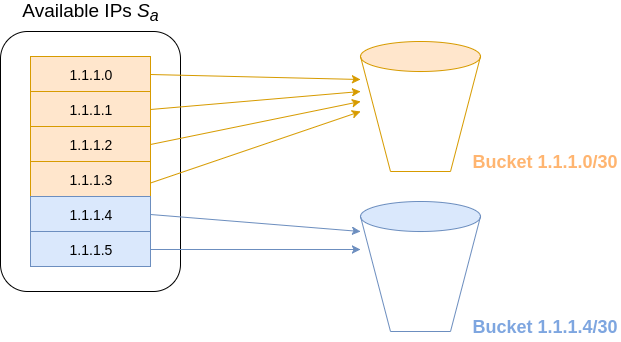
\includegraphics[width=0.7\textwidth]{renders/IpsByBucketSize4.png}
      \caption{Assigning IPs to Buckets with a Bucket Size of 4}
      \label{fig:exampleIpsByBucket4}
\end{figure}

As discussed, the bucket size will be an integral power of 2, but an important question is which integral power of 2. The algorithm starts by assigning the IPs to their buckets using a bucket size equal to the largest possible CIDR block that can be obtained for the given $t$. As discussed previously, this is the largest integral power of 2 that is less than or equal to $t$.

At this point, the algorithm begins to take shape. Consider the situation represented in \reffig{fig:exampleIpsByBucket4} along with a value of $t = 4$. The initial bucket size will be 4 and the presence of a filled bucket ($1.1.1.0/30$) indicates that a CIDR block of the bucket size can be created. Since the bucket size is equal to the desired number of IPs, the optimal choice is the $1.1.1.0/30$ block. The algorithm can return this block and it will be the optimum set of addresses to choose to minimize the number of CIDR entries required to represent the set of IP addresses.

Next consider the situation represented in \reffig{fig:exampleIpsByBucket4} along with a value of $t = 6$. The initial bucket size will still be 4 (as this is the largest integral power of 2 less than or equal to $t$). Thus, the algorithm will again detect that the $1.1.1.0/30$ bucket is full and select this block of four IPs. However the algorithm must return a total of $t = 6$ IPs and therefore must select a further 2 IPs. The algorithm accomplishes this by making a recursive call. By removing all of the (so far) selected IPs from the set of available IPs (forming $S_a'$, the \textit{available} set for the next call) and setting the new value of $t$ to be the remaining number of IPs required ($t'$ = 2), a recursive call will simply find the best set of IPs from what is left. This is shown in \reffig{fig:exampleIpsByBucket2} in which the recursive call would return $1.1.1.4/31$ as this bucket is full. The selected IPs from each recursive call are then unioned, returning the optimum set of IPs - $\{1.1.1.0/30,\enspace1.1.1.4/31\}$

\begin{figure}[H]
      \centering
      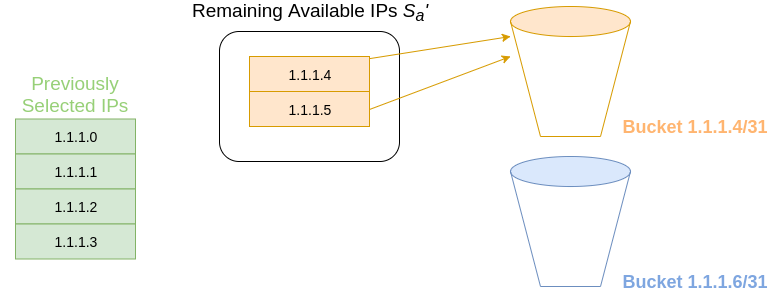
\includegraphics[width=0.8\textwidth]{renders/IpsByBucketSize2.png}
      \caption{Assigning Remaining IPs to Buckets with a Bucket Size of 2}
      \label{fig:exampleIpsByBucket2}
\end{figure}

In the case of $t = 7$, the algorithm would proceed as before, with one extra recursive call with $t = 1$. Assuming there were sufficient IPs available (the number of IPs in the diagrams were limited for brevity), the algorithm would have selected the same 6 IPs as before and the final call would be the trivial case of $t = 1$ in which a random IP can be selected. At each stage, the set of IPs returned from the recursive calls can then be unioned with the current call's chosen IPs, and the unioned set returned. 

The final possibility to consider is what should be done when no buckets are filled. In this case, the algorithm should not select any IPs at this bucket size. Instead, it should reduce the bucket size to the next highest integral power of 2 and recurse, setting $t$ equal to this reduced bucket size. However, there is another important step, the need for which is best illustrated with an example. A diagram of this situation is shown in \reffig{fig:ipAlgTrickyCodePath}

If the initial value for $t$ is 6, the initial bucket size will be 4. If no buckets of size 4 are filled, the algorithm will then recurse. Let this recursive call be denoted as $r_1'$, where $'$ indicates the depth of the recursion. Let the total number of IPs required for this recursive call $r_1'$ be denoted as $t_1'$. Thus, $t_1' = 2$ (the next largest integral power of 2 as discussed previously) and the set of available IPs is unchanged $S_{a_1}' = S_a$. Let the set of chosen IPs returned from $r_1'$ be denoted as $S_{c_1}'$.

The initial call required 6 IPs to be returned and $r_1'$ will return the 2 green IPs shown in \reffig{fig:ipAlgTrickyCodePath}, $\{1.1.1.0,\enspace1.1.1.1\}$. Thus, a second recursive call, $r_2'$ is required. This recursive call, $r_2'$ is \textbf{not} nested within the first recursive call $r_1'$, but rather is a sibling recursive call (it is at the same depth as $r_1'$).  Let the total number of IPs required for $r_2'$ be denoted as $t_2'$. $t_2'$ is calculated using the formula given in \refeq{eq:secondRecurseT2}. This is simply the remaining number of IPs that need to be chosen after the first recursive call. In this case, $t_2' = 6 - 2 = 4$. 

\begin{equation}\label{eq:secondRecurseT2}
t_2' = t - t_1'
\end{equation}

The set of available IPs that is used for $r_2'$, $S_{a_2}'$, is given by \refeq{eq:availableIpsSecondRecurse}. This is the initial set of all available IPs, with the IPs chosen from the first recursive call omitted. Let the set of IPs returned from $r_2'$ be denoted as $S_{c_2}'$.

\begin{equation}\label{eq:availableIpsSecondRecurse}
S_{a_2}' = S_a - S_{c_1}'
\end{equation}

\begin{figure}[H]
      \centering
      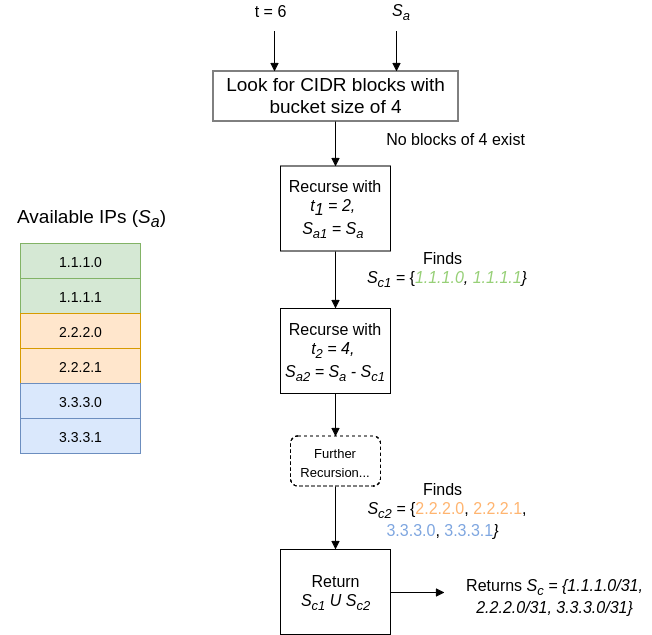
\includegraphics[width=\textwidth]{renders/IpAlgTrickyCodePath.png}
      \caption{Code Path When Algorithm Does Not Find Full Bucket}
      \label{fig:ipAlgTrickyCodePath}
\end{figure}

The second recursive call, $r_2'$ (as described above), will then look for IPs using a bucket size of 4. Again, none will be found. Thus, the algorithm will need to recurse again. Let this call be denoted $r_1''$. The bucket size for $r_1''$ will be 2 (the next highest integral power of 2). Thus, $r_1''$ will find the 2 IPs shown in orange in \reffig{fig:ipAlgTrickyCodePath}, $\{2.2.2.0,\enspace2.2.2.1\}$. However the second recursive call $r_2'$ required a total of 4 IPs and only 2 have been selected. Thus, just as in the first case, a sibling recursive call, $r_2''$ is required to choose the remaining IPs. Thus, $r_2''$ will require two more IPs to be chosen and will return the blue set of IPs shown in \reffig{fig:ipAlgTrickyCodePath}, $\{3.3.3.0,\enspace3.3.3.1\}$. The union of the results of $r_1''$ and $r_2''$ will be returned to $r_2'$ and will contain the required 4 IPs, $\{2.2.2.0/31,\enspace3.3.3.0/31\}$. Finally, the result of $r_1'$ and $r_2'$ will be unioned, returning the desired 6 IPs, $\{1.1.1.0/31,\enspace2.2.2.0/31,\enspace3.3.3.0/31\}$.

Now that all cases have been considered, the steps of the algorithm (for the simplified case of having no existing IPs) are shown below:
\begin{itemize}
\item{Set bucket size to the largest integral power of 2 that is less than or equal to $t$}
\item{Assign all available IPs into buckets using the calculated bucket size}
\item{If a bucket is full}
  \begin{itemize}
  \item{Add all the IPs in the bucket to the set of chosen IPs ($S_c$)}
  \item{Remove all the IPs in the bucket from the set of available IPs (forms $S_a'$)}
  \item{Calculate $t'$ as $t - bucketSize$}
  \item{Recurse using $S_a'$ and $t'$ (if necessary)}
  \end{itemize}
\item{Otherwise}
  \begin{itemize}
  \item{Recurse ($r_1'$) using next biggest integral power of 2 and the initial set of available IPs}
  \item{Recurse again ($r_2'$) using the remaining number of IPs required and the set of available IPs, excluding those returned from $r_1'$ ($S_{c_1}'$)}
  \item{Return the union of the results of the two recursive calls.}
  \end{itemize}
\end{itemize}

\subsection{Extending the Algorithm to Support Existing IPs}
Now that a solution to the simplified problem where $S_e = \{\}$ has been formed, the more complex initial problem could now be tackled. However upon closer inspection, there is only one extra point to consider when the set of existing IPs is non empty: \textbf{the final set must be a super set of the set of existing IPs}. 

The extended algorithm's parameters are changed to the following to aid in the recursion:

\begin{itemize}
\item{A list of available IPs - $S_a$}
\item{A list of existing IPs - $S_e$}
\item{The total number of IPs desired - $t$}
\item{The bucket size to use - $b$}
\end{itemize}

The main changes to the algorithm are the following:

\begin{itemize}
  \item{Assign the existing IPs ($S_e$) to buckets using the provided bucket size}
  \item{Assign the available IPs ($S_a$) to separate buckets using the provided bucket size}
  \item{For each of the \textit{existing} IP buckets $S_{e_i}$}
      \begin{itemize}
      \item{Calculate $b^*_i$, the number of IPs required to fill the bucket (\refeq{eq:ipsToFillBucket})}
      \item{If the number of IPs in the corresponding \textit{available} IP bucket ($S_{a_i}$) equals $b^*_i$, the union of the two buckets creates a CIDR block and should be added to the currently chosen set of IPs ($S_c$), as long as it doesn't cause $|S_c|$ to become larger than the total number of desired IPs, $t$}
      \item{If $|S_c|$ is now equal to $t$ (the total number of IPs required), $S_c$ can be returned.}
      \item{Otherwise, recurse (see below)}
      \end{itemize}
\end{itemize}


\begin{equation}\label{eq:ipsToFillBucket}
b^*_i= b-|S_{e_i}|
\end{equation}


This shows that the only logical change is that the number of IPs required to \textit{fill the existing IP buckets} should be examined, rather than searching for full buckets from the available pool. 

As with the simplified case, this method may require some recursion after the above steps. The recursive call in this case is actually simpler, but depends on the current state of the algorithm. As previously mentioned, all the IPs in the existing set should be contained in the final set. If the algorithm reaches a state where all the existing IPs have been used, but there is still a number of IPs to be selected, the algorithm can simply fallback to the previous case where $S_e = \{\}$. 

Otherwise, the algorithm recurses using the remaining available IPs, the remaining \textit{required} IPs (this is the set of existing IPs that have not yet been chosen), the remaining number of IPs to be chosen and the next bucket size to use which is the next largest integral power of 2.

Consider the following example as shown in \reffig{fig:ipsByBucketExisting4}.
\begin{itemize}
\item{$S_e = \{1.1.1.0,\enspace2.2.2.0\}$}
\item{$S_a = \{1.1.1.1,\enspace1.1.1.2,\enspace1.1.1.3,\enspace2.2.2.1,\enspace2.2.2.2\}$}
\item{$t = 7$}
\end{itemize}

As $t = 7$, the initial bucket size $b$ would be 4 and the IPs would be assigned to buckets as shown in \reffig{fig:ipsByBucketExisting4}

The algorithm would then proceed in the following manner:
\begin{itemize}
\item{Examine each existing bucket ($S_{e_i}$) and the corresponding available bucket ($S_{a_i}$)}
\begin{itemize}
\item{Calculate $b_i^*$ for $1.1.1.0/30$ as per \refeq{eq:ipsToFillBucket}, yielding 3}
\item{Add $1.1.1.0/30$ to $S_c$ as $b^*_i = |S_{a_i}| = 3$}
\end{itemize}
\begin{itemize}
\item{Calculate $b_i^*$ for $2.2.2.0/30$ as per \refeq{eq:ipsToFillBucket}, also yielding 3}
\item{Skip $2.2.2.0/30$ as $b^*_i > |S_{a_i}|$ ($3 > 2$)}   
\end{itemize}
\end{itemize}

\begin{figure}[H]
      \centering
      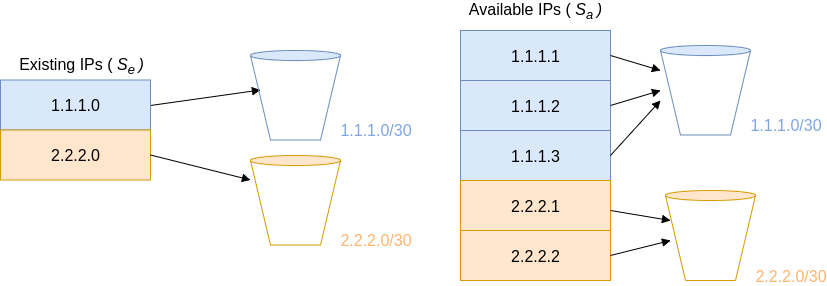
\includegraphics[width=0.8\textwidth]{renders/IpsByBucketSize4Existing.png}
      \caption{Available and Existing IPs Assigned to Buckets of Size 4}
      \label{fig:ipsByBucketExisting4}
\end{figure}

Since the total number of IPs required was $t = 7$ and only 4 IPs have been selected, a recursive call is required. As there are still some existing IPs that have not been included, a recursive call is made with the following parameters:
\begin{itemize}
\item{$S'_e = \{2.2.2.0\}$ - the remaining \textit{required} IPs that have not yet been chosen}
\item{$S'_a = \{2.2.2.1,\enspace2.2.2.2\}$ - the remaining \textit{available} IPs}
\item{$t' = 3$ - the remaining \textit{number} of IPs to be selected}
\item{$b' = 2$ - the bucket size should be the next largest integral power of 2 (was 4)}
\end{itemize}

Thus, the IPs will be assigned to buckets of size 2, as shown in \reffig{fig:ipsByBucketExisting2}.

The algorithm will then proceed as follows:
\begin{itemize}
\item{Examine each existing bucket ($S_{e_i}'$) and the corresponding available bucket ($S_{a_i}'$)}
\begin{itemize}
\item{Calculate $b*'_i$ for $2.2.2.0/31$ as per \refeq{eq:ipsToFillBucket}, yielding 1}
\item{Add $2.2.2.0/31$ to $S_c'$ as $b*'_i = |S'_{a_i}| = 1$} 
\item{Skip $2.2.2.2/31$ as $b*'_i > |S'_{a_i}| (2 > 1)$}
\end{itemize}
\end{itemize}

\begin{figure}[H]
      \centering
      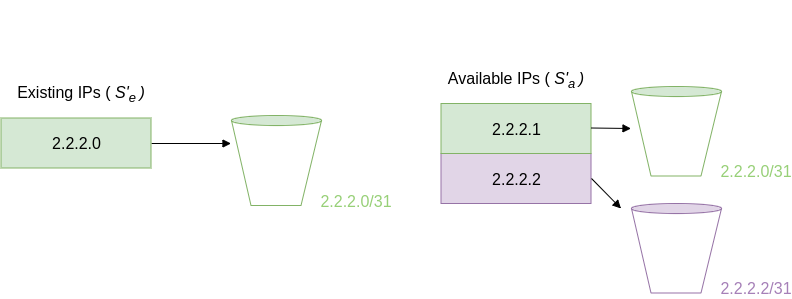
\includegraphics[width=0.8\textwidth]{renders/IpsByBucketSize2Existing.png}
      \caption{Remaining Available and Existing IPs Assigned to Buckets of Size 2}
      \label{fig:ipsByBucketExisting2}
\end{figure}

Finally, since a total of 7 IPs were required and 6 have now been selected, a final recursive call is required. However all the existing IPs have now been chosen, meaning the existing IPs argument for the next recursive call will empty. This means the algorithm falls back to the simple case as described earlier and will choose a random final IP ($2.2.2.2$ in this case). 

There are two enhancements that can be made to the algorithm at this point.

\begin{enumerate}
\item{A better method for choosing a \textbf{single} IP from the available IP pool. This shouldn't be done randomly as this could result in large CIDR blocks contained in the available IP pool being broken up unnecessarily. This is described in \refapp{appendix:smartSingleIP}.}
\item{In the case where the existing set of IPs ($S_e$) is non empty, the previously described method of choosing the highest integral power of 2 that is less than or equal to $t$ for the initial bucket size is not ideal. Given a set of 2 IPs and requiring a total of 4 IPs, the approach would suggest starting with a bucket size of 4. However unless the existing IPs themselves are contiguous, there is no possibility of forming a CIDR block of size 4. This is described in detail in \refapp{appendix:smartInitBucket}.}
\end{enumerate}

Finally, the entire source code for the algorithm can be found in \refapp{appendix:cidrMinSource}

\break

\subsection{Unit Testing the Algorithm}
The final step in the development was to write extensive unit tests to ensure the algorithm operates as expected. Unit testing is an critical part of the software development process at HubSpot and engineers are always encouraged to write code which is as unit testable as possible. As the code is essentially a number of static utility functions, unit testing is quite simple and does not require mocking any complex objects.  

The initial task was to come up with an example state to test the algorithm with. The example state contains the set of available IP addresses $S_a$ and the set of existing IP addresses $S_e$. These should be chosen in such a way that all code paths of the algorithm are seen at some point or another when running the tests. This requires some consideration as for what is contained in $S_a$ and $S_e$, as well as the total number of IPs required, $t$, for each of the test cases.

As a starting point, the following sets of IPs were chosen for the default state (this can be changed on a per test basis of course):

\begin{equation}\label{eq:initialState}
\begin{gathered}
S_a = \{1.1.1.2,\enspace1.1.1.3,\enspace1.1.1.4,\enspace1.1.1.5,\enspace1.1.1.6,\enspace1.1.1.7,\enspace1.1.1.8,\enspace1.1.1.9\} \\
S_e = \{1.1.1.0,\enspace1.1.1.1\}
\end{gathered}
\end{equation}

Initially however, tests were written for the simplified case where $S_e = \{\}$. The following tests were then implemented:

\begin{itemize}
\item{The algorithm should choose contiguous blocks when available}
      \begin{itemize}
      \item{This was tested by simply requesting that 4 IPs be selected from $S_a$ and ensuring that the resulting set was $\{1.1.1.4/30\}$.}
      \end{itemize}
\item{The algorithm should find contiguous blocks of IPs when a single IP will be left over}
      \begin{itemize}
      \item{This was tested by requesting that 5 IPs be selected from $S_a$}
      \item{The resulting set should contain the block of 4 IP addresses ($1.1.1.4/30$) and a single other IP}
      \item{This test was added to ensure that the algorithm still selected a block of four instead of trying to find several blocks of 2}
      \end{itemize}
\item{The algorithm should find contiguous IPs recursively}
      \begin{itemize}
      \item{This was tested by requesting that 6 IPs be selected from $S_a$}
      \item{The resulting set should contain the block of 4 IP addresses ($1.1.1.4/30$) as before, but should also select the $1.1.1.2/31$ block for the remaining 2 IP addresses}
      \item{This test was sufficient to assume the algorithm would recursively select CIDR blocks at lower block sizes when available}
      \end{itemize}
\item{The algorithm should always return the correct number of IP addresses}
      \begin{itemize}
      \item{This test was implemented by repeatedly invoking the algorithm with $t$ running from $1$ to $|S_a|$ and ensuring $|S_c| = t \enspace \forall \enspace t$}
      \end{itemize}
\end{itemize}

These tests were sufficient for the simple case where $S_e = \{\}$ and the algorithm was then tested using the more complex case. The following tests were implemented in order to ensure correctness of the algorithm:

\begin{itemize}
\item{The algorithm should find contiguous blocks when provided with existing IP addresses}
      \begin{itemize}
      \item{This was tested by requesting a total of 4 IPs, given the default state as described in \refeq{eq:initialState}}
      \item{The algorithm should then select $\{1.1.1.2/31\}$} so that when unioned with $S_e = \{1.1.1.0/31\}$, the CIDR block $\{1.1.1.0/30\}$  is formed 
      \end{itemize}
\item{The algorithm should always return the correct number of IPs and contain all the existing IPs}
      \begin{itemize}
      \item{This test was an important test as the algorithm would be useless if it minimized CIDR blocks but didn't guarantee that all of the existing IPs would be present in the resulting set}
      \item{This test was implemented by allowing a variable $i$ to take on values from $1$ to $|S_a|$ and by setting $t = |S_e| + i$.}
      \item{This essentially repeatedly runs the algorithm, requesting each possible value from the minimum number of new IPs (1), to the maximum number of new IPs (the number of available IPs)}
      \item{At each iteration, the returned set was checked to ensure the correct number of IPs was returned and that all of the existing IPs were contained in that set.}
      \end{itemize}
\item{The algorithm was also tested to ensure it would look for contiguous blocks both above and below (in the IP address space) the existing IPs provided in order to try and find CIDR blocks}
      \begin{itemize}
      \item{This was tested by requesting a total of 2 IPs and setting $S_e = \{1.1.1.3\}$}
      \item{This tested that the algorithm would find CIDR blocks below the existing IPs provided}
      \item{The algorithm should return $1.1.1.2/31$, indicating it correctly searches below the provided existing IPs}
      \item{A similar test was written where $S_e = {1.1.1.2}$ and the algorithm correctly returned $1.1.1.2/31$ indicating that it also looks above the provided existing IP addresses for CIDR blocks}
      \end{itemize}
\item{The algorithm should find CIDR blocks with existing IP addresses that cause a single IP to be left over}
      \begin{itemize}
      \item{This was tested by requesting a total of 9 IPs using the default state as shown in \refeq{eq:initialState}}
      \item{The resulting set should contain the CIDR block of 8 IPs ($1.1.1.0/29$) and the remaining extra IP ($1.1.1.9$)}
      \end{itemize}
\item{The algorithm should return already grouped existing IPs}
      \begin{itemize}
      \item{It is essentially impossible to break up a CIDR block contained inside the set of existing IP addresses, but this test was added to ensure the algorithm correctly identified existing CIDR blocks appropriately.}
      \item{A set of existing IPs $S_e = \{2.2.2.0/31\}$ was used along with an the available set of IPs listed in \refeq{eq:initialState} and a total of 4 IPs were requested.}
      \item{The algorithm correctly returned the existing CIDR block as well as another CIDR block of size 2, yielding $\{1.1.1.2/31,\enspace2.2.2.0/31\}$}
      \item{This ensured the algorithm selected the existing block of 2 as well as another block of 2, instead of selecting a block of 4 by excluding existing IPs}
      \end{itemize}
\item{The algorithm should handle existing IPs which don't contribute to any CIDR blocks and should fill the remaining number of IPs required with the best CIDR block from the available set of IPs}
      \begin{itemize}
      \item{This was tested by setting $S_e = \{2.2.2.0,\enspace3.3.3.0,\enspace4.4.4.0\}$}, using the set of available IPs shown in \refeq{eq:initialState} and requesting 5 IPs.
      \item{The algorithm should then return the three existing IPs along with a CIDR block of size 2 from the set of available IPs}
      \end{itemize}
\end{itemize}

These tests provided a sufficient amount of coverage to provide confidence in the algorithm and its implementation. Several other tests were implemented which were less specific to the algorithm (such as ensuring user input was validated). The algorithm has been running in a production environment for over 3 months and has helped automate an important step that was previously being performed manually by a support team at HubSpot.   

\section{Abstracting Upstream Email Sending to Kafka}
While discussing Kafka in \refsec{sec:kafka}, an idealized case of having all emails that need to be sent through HubSpot simply placed on a Kafka topic was shown. This functionality is supported for emails that can be sent through HubSpot's internal Mail Transfer Agent (MTA) (see \refsec{sec:emailSendingInfra} for more details), but is not supported for emails using other third party MTAs. The reason for this was HubSpot's email marketing was initially built using third party MTAs, prior to the development of the internal MTA. Prior to this task, email sent through third party MTAs was done \textit{in-process}, inside of an upstream email team's deployable, as all of this code was written prior to the formation of the \team{} team. This code is entirely to do with email sending and thus should certainly be owned and controlled by the \team{} team. It also adds a considerable amount of latency to the upstream email team's code, as they must wait for the results of email sends. 

The main goal of this task was to decouple the email sending code from the upstream teams deployable. Kafka was the perfect choice to use as the interface between the two teams and the desired setup was for the upstream team to produce the emails to be sent to a given Kafka topic, for those emails to be sent by the \team{} team's Kafka consumers and for the results of the email send to be produced back to the upstream email team through a second Kafka topic.

The major difficulty associated with rewriting the code in this way was that the results of the email send were no longer obtainable in-process of the upstream teams deployable. The email sending would essentially happen asynchronously and the results would be present in a \textbf{different} deployable. Ultimately this is the exact behavior that is desired as the process producing these emails to Kafka should be able to \textit{"fire and forget"} - once it has produced the email to Kafka, it has done its job.

The main difficulty associated with this task was implementing the solution in a \textit{backwards compatible} way. All of HubSpot's outgoing marketing email would be run through this new code path. Thus, it must be rolled out extremely slowly and carefully. This meant the code changes must be made in such a way that either the old in-process email sending, or the new Kafka email sending could be used. 

This task was essentially two tasks which were entirely dependent on one and other. One of these tasks was creating the infrastructure required on the \team{} team's side of things and the other was making use of this infrastructure on the upstream email team's side of things.
\break

\subsection{The \team{} Team's Side}
This task required the creation of an entirely new project owned by the \team{} team. This project would now contain all the code required for sending the emails to both the internal MTA and the third party MTAs. This required substantial research into setting up and configuring Kafka and setting up a project on the HubSpot stack. 

As discussed, all changes had to be backwards compatible. This was achieved by writing a new higher level abstraction of a class which sends emails. To the upstream team, they would simply obtain a reference to an object which had a \java{produceEmailRequest} method. Under the hood, there were several implementations of an interface which contained this method. One of these implementations provided access to the old in-process email senders, while the other implementations provided access to the new Kafka producers which would produce these emails to the new Kafka topic. This abstraction was provided to the upstream team, allowing the \team{} team to control \textit{under what circumstances} and \textit{when} the new Kafka sending pipeline could be used. For example, the Kafka senders could be used a configurable number of times per minute, for particular types of email sends, or disabled entirely.

This extra consideration and layer of abstraction was key in providing a mechanism for safely rolling out changes which could potentially break \textbf{every} email that was to be sent through HubSpot.

\subsection{The Upstream Email Team's Side}
The upstream email team in this case were the team responsible for managing all the data generated around an email to be sent. In this circumstance, their main task was performing all the required work that was to be done post send attempt. This included writing the email to a variety of places, producing events which lead to customer billing, tracking the number of sends a particular customer had made and many others. 

The main issue at this point was some of this \textit{post-send} logic required the \textbf{result} of the email send. However as the main purpose of this task was to decouple the email send from their process and reduce latency, by definition, the results of email sends were no longer available. This required careful splitting out of the \textit{post-send} logic into what could be performed in-process and what could not. Any of the logic which was entirely dependent on the result of the email send had to be moved into a Kafka consumer, listening to the results of the email sends, which were produced by the \team{} team's Kafka consumers who were responsible for sending the email.

Though the task may seem trivial, this was actually one of the most difficult tasks undertaken throughout the course of the internship. A monumental amount of research and consideration was required in order to ensure all edge cases were covered and that the new Kafka sending pipeline would be stable. As discussed, every marketing email sent through HubSpot would run through this code and this code was also responsible for billing customers, so any bugs could have proved extremely costly.

